\documentclass{article}
\usepackage{graphicx}
\usepackage{textcomp,gensymb}
\usepackage{amssymb}
\usepackage{enumitem}
\usepackage{amsmath}
\usepackage{marvosym}
\usepackage{siunitx}

\begin{document}
 \title{GATE}
 \author{BHUVANA}
 \maketitle

 \begin{enumerate}
 \item

	 Consider the $2$-bit multiplexer(MUX) shown in the figure. For OUTPUT to be the XOR of C and D, th values for $A_0$,$A_1$,$A_2$ and $A_3$  are \underline{\hspace{50pt}}
	 \begin{figure}[h]
		 \centering
		 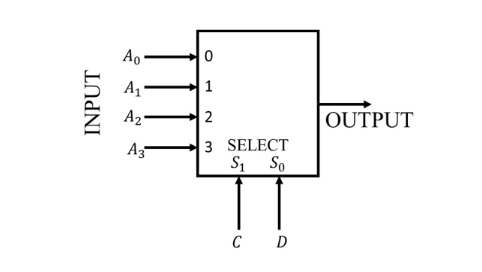
\includegraphics[width=\columnwidth]{pics/gatepic.jpg}
		 \label{fig:MUX}
	\end{figure}
	 \begin{enumerate}[label=(\Alph*)]
		\item $A_0=0,A_1=0,A_2=1,A_3=1$
		\item $A_0=1,A_1=0,A_2=1,A_3=0$
		\item $A_0=0,A_1=1,A_2=1,A_3=0$
		\item $A_0=1,A_1=1,A_2=0,A_3=0$
	\end{enumerate}
 \end{enumerate}
\end{document}

